\documentclass{article}
\usepackage{xcolor}
\usepackage[final]{wod_alpasim_2026}

\usepackage{amsmath}
\usepackage{booktabs}
\usepackage{graphicx}
\usepackage{microtype}
\usepackage{hyperref}
\usepackage{tikz}
\usetikzlibrary{arrows.meta,positioning}
\raggedbottom

\title{WOD2Sim: Adapting WOD-Style Driving Policies\\
to Closed-Loop AlpaSim Evaluation}

\author{
  Alba Maria Tellez Fernandez\\
  \texttt{amtellezfernandez@gmail.com}
}

\hypersetup{
  pdftitle={WOD2Sim: Adapting WOD-Style Driving Policies to Closed-Loop AlpaSim Evaluation},
  pdfauthor={Alba Maria Tellez Fernandez},
  pdfsubject={WOD2Sim manuscript 2026}
}

\begin{document}

\maketitle

\begin{abstract}
AlpaSim has a plugin mechanism for trajectory models, but its stock external-driver
contract was not sufficient for Waymo Open Dataset (WOD)-style policies. The driver input
reduced route updates to a command before prediction, while our policies needed local
route waypoints. Model discovery could import Alpamayo or VAM before an external driver
was selected. Closed sessions could still receive image, egomotion, route, or close
messages. Local runs depended on Hydra, Docker, GPU runtime, scene-artifact, and checkout
state that was not recorded with the experiment. We call the resulting adapter
\emph{WOD2Sim}; it extends the AlpaSim
external-driver contract at these four points: route geometry, model discovery, session
lifecycle, and launch state. The implementation patches \texttt{PredictionInput} and the
driver session, makes built-in model imports lazy, treats late session messages
idempotently, registers three project policies through \texttt{alpasim.models}, converts
AlpaSim prediction inputs into policy-facing route and scene signal, and provides setup,
readiness, launch, and validation commands. The contribution is not a new driving policy
or a log converter. WOD2Sim defines and validates an adapter contract that turns
WOD-style logged-policy evaluation into auditable closed-loop execution inside AlpaSim.
\end{abstract}

\section{Introduction}

The Waymo Open Dataset (WOD) end-to-end driving task and AlpaSim solve different
problems, so they expose different interfaces. WOD gives a policy-learning contract:
observe camera and ego context, condition on route intent, and predict a short-horizon
trajectory~\citep{sun2020scalability}. AlpaSim gives a simulator-execution contract: a
live driver service is discovered as a trajectory-model plugin, receives camera and
egomotion messages over time, processes route updates, returns trajectory points and
headings at the rollout clock, and remains alive inside a distributed runtime~\citep{alpasim2026}.

That difference is the reason a direct policy wrapper was insufficient. A dataset policy
usually expects a compact, already-assembled example. A simulator driver must survive an
ongoing session and consume state as it arrives. In stock AlpaSim, route geometry had
already been collapsed into a left/straight/right command before prediction, which is
acceptable for command-conditioned models but not for policies that score trajectories
against a local route polyline. Even after route waypoints were exposed, another mismatch
appeared: multi-lane road centers were not necessarily ego travel lanes. The remaining
gaps were also between a dataset contract and a simulator contract: importing the model
package could require unselected Alpamayo or VAM backends, late session messages could
terminate batch runs, and launch assumptions lived outside the experiment record.

This paper is about extending that simulator-side contract so WOD-style policies can run
as ordinary AlpaSim external drivers. WOD2Sim preserves route geometry at
prediction time, decouples external plugin discovery from unrelated built-in backends,
makes session handling idempotent under normal service ordering, and records launch state
before rollout. On top of that contract, the project registers a reflex policy, a learned
token BC/DAgger policy, and a direct actor-aware planner through
\texttt{alpasim.models}, reconstructs a policy-facing signal from AlpaSim inputs, and
provides setup, readiness, launch, and validation commands. The artifact claim is narrow:
this is not a new autonomy method, but a reusable external-driver contract extension for
turning dataset-style trajectory policies into executable AlpaSim drivers.

The contributions are:
\begin{itemize}
\item an AlpaSim external-driver contract extension for WOD-style trajectory policies,
including route geometry, trajectory resampling, and policy-facing scene signal;
\item simulator-runtime hardening for lazy model discovery, late session messages, and
idempotent close behavior that would otherwise corrupt batch evaluation;
\item launch-state materialization and readiness checks for reproducing runs under local
Docker, GPU, scene-artifact, and checkout constraints;
\item an evidence pipeline that emits manifests, audits, support-bundle reports, hashes,
and benchmark summaries while avoiding redistribution of gated assets.
\end{itemize}

\section{External-Driver Contract Gaps}

Stock AlpaSim already has the right outer loop: the runtime asks an ego-driver service
for a trajectory, and the controller executes it. The failure was inside that loop. The
driver input did not carry the route geometry our policies used, model discovery pulled
in built-in backends before our plugin was selected, and the service treated normal late
messages as fatal unknown-session errors. Launch state was also distributed across
Hydra, Docker, GPU runtime, and scene-artifact assumptions. Table~\ref{tab:stock_vs_adapted}
lists the contract points we had to change.

\begin{table}[t]
\centering
\small
\begin{tabular}{p{0.23\linewidth}p{0.31\linewidth}p{0.34\linewidth}}
\toprule
Contract point & Stock AlpaSim behavior & WOD2Sim behavior \\
\midrule
Route input & route used mainly for command & route waypoints preserved for prediction \\
Model imports & eager built-in backend imports & lazy imports for external plugin envs \\
Plugin boundary & built-in model stack & local \texttt{alpasim.models} policies \\
Session messages & unknown-session errors & late messages handled idempotently \\
Trajectory output & simulator frequency contract & WOD-style 5 s horizon resampled to runtime \\
Deployment & wizard-driven built-ins & matched external driver and wizard commands \\
Host setup & monolithic dependency assumptions & minimal editable install and overrides \\
\bottomrule
\end{tabular}
\caption{External-driver contract gaps exposed by WOD-style policies. The adapter keeps
AlpaSim's driver loop but extends the state available at its boundary.}
\label{tab:stock_vs_adapted}
\end{table}

\subsection{Route Geometry Must Survive Prediction}

Stock AlpaSim and WOD-style policies do not consume equivalent route representations. In
the original driver API, \texttt{PredictionInput} contained camera images, command,
speed, acceleration, and ego pose history. The route had already been reduced to a
high-level driving command such as left, straight, or right. That abstraction is
sufficient for command-conditioned models, but it discards the local waypoint geometry
needed by policies that generate trajectory points relative to a route centerline.

This loss cannot be repaired downstream in policy code. Once the route
has been reduced to a command, the polyline geometry that distinguishes two legal left
turns, lane offsets, curvature, and local alignment is no longer available to the model.
The required change is therefore an extension of the simulator-facing prediction
contract: route waypoints must remain available at prediction time.
Figure~\ref{fig:contract_patch} shows this contract change. The command remains available, but
the route waypoints are preserved as first-class model input rather than reconstructed
from a categorical intent symbol.

The implementation also exposed a second route error: a road centerline is not always
the ego travel lane. In multi-lane scenes, scoring trajectories against the geometric
road center can make a legal ego lane appear laterally offset or unsafe. The adapter
therefore treats route waypoints as the policy route and derives route-centered lane
geometry for policy scoring, instead of assuming that the simulator's visual road center
is the trajectory reference.

\begin{figure}[t]
\centering
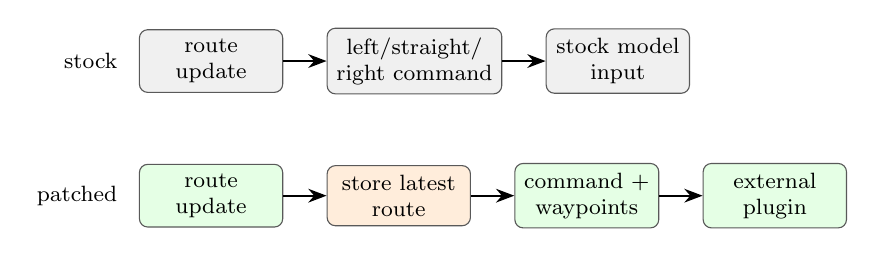
\begin{tikzpicture}[
  node distance=0.5cm and 0.55cm,
  box/.style={rectangle,rounded corners=3pt,draw=black!65,minimum height=0.62cm,
              minimum width=1.82cm,font=\footnotesize,align=center},
  stock/.style={box,fill=gray!12},
  patched/.style={box,fill=green!10},
  store/.style={box,fill=orange!14},
  arr/.style={-Stealth,thick}
]
  \node[stock] (route_a) {route\\update};
  \node[stock,right=of route_a] (cmd_a) {left/straight/\\right command};
  \node[stock,right=of cmd_a] (model_a) {stock model\\input};

  \node[patched,below=0.9cm of route_a] (route_b) {route\\update};
  \node[store,right=of route_b] (store_b) {store latest\\route};
  \node[patched,right=of store_b] (input_b) {command +\\waypoints};
  \node[patched,right=of input_b] (plugin_b) {external\\plugin};

  \draw[arr] (route_a) -- (cmd_a);
  \draw[arr] (cmd_a) -- (model_a);
  \draw[arr] (route_b) -- (store_b);
  \draw[arr] (store_b) -- (input_b);
  \draw[arr] (input_b) -- (plugin_b);

  \node[font=\footnotesize,align=right,left=0.15cm of route_a] {stock};
  \node[font=\footnotesize,align=right,left=0.15cm of route_b] {patched};
\end{tikzpicture}
\caption{The key AlpaSim driver-contract patch preserves route waypoints for prediction
instead of reducing route input to a command-only signal.}
\label{fig:contract_patch}
\end{figure}

\subsection{Model Discovery Must Not Import Unselected Backends}

The second incompatibility is in model discovery. Stock AlpaSim's model package assumes
that built-in learned-driver backends are available when the package is imported. That is
reasonable for the simulator's native stack, but it breaks the external-driver case. A
local WOD-style plugin may need only \texttt{BaseTrajectoryModel}, \texttt{PredictionInput},
and the \texttt{alpasim.models} entry point. If those imports also load Alpamayo or VAM,
the driver can fail before the requested external model is selected.

WOD2Sim therefore separates the stable base contract from heavyweight backend
availability. The important claim is not that lazy loading is more convenient; it is that
external driver execution requires \texttt{BaseTrajectoryModel},
\texttt{PredictionInput}, \texttt{ModelPrediction}, and related base types to be
importable without installing every built-in model backend. This makes the plugin
boundary explicit: external policies can register through the same AlpaSim mechanism as
native models while depending only on the driver contract they actually use.
This is not a claim that the AlpaSim driver is torch-free; the setup path still installs
torch for the driver environment. The removed coupling is to unrelated built-in policy
backends that are not needed by a selected external plugin.

\subsection{Session Lifecycle Must Be Idempotent}

The third incompatibility appears only once the code runs as a simulator service. A
script-style converter can assume one ordered control flow. AlpaSim rollouts involve a
runtime, driver service, controller, renderer, and deployment orchestration exchanging
session-scoped messages asynchronously. Duplicate closes and late image, egomotion, or
route messages are normal service-lifecycle events, not necessarily policy failures.

Treating those messages as fatal unknown-session errors makes closed-loop batch
evaluation fragile for reasons unrelated to policy quality. The driver service must
therefore make session handling idempotent at the runtime boundary: late messages should
be recorded as controlled warnings and ignored when their session is no longer active.
Without this session behavior, repeated external-driver runs fail for service-lifecycle
reasons rather than for policy errors.

\subsection{Launch State Must Be Materialized}

The final contract gap is outside the model API. A local AlpaSim external-driver run
depends on a matched driver command, wizard command, topology, base port, scene IDs,
Docker image, GPU runtime, platform constraints, and gated scene artifacts. If those
values live only in shell history or ad hoc Hydra overrides, the policy cannot be
re-executed as a reviewable artifact. WOD2Sim therefore treats launch state as part
of the external-driver contract: setup checks plugin discovery, readiness checks runtime
preconditions, and print mode emits the exact driver and wizard commands before rollout.

\section{Implemented Contract}

Figure~\ref{fig:architecture} shows the implemented contract boundary. The implementation
has two halves: changes inside the AlpaSim checkout, and project code that behaves like
ordinary AlpaSim model plugins.

\begin{figure}[t]
\centering
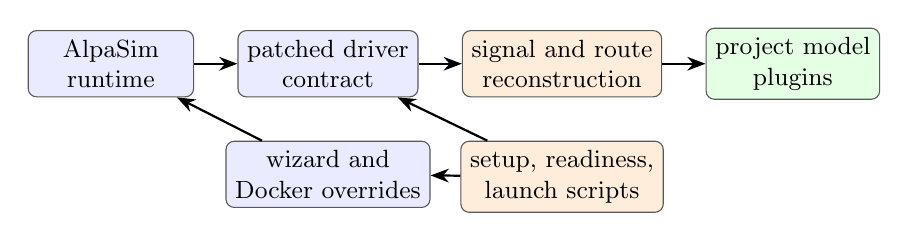
\begin{tikzpicture}[
  node distance=0.55cm and 0.55cm,
  box/.style={rectangle,rounded corners=3pt,draw=black!65,minimum height=0.72cm,
              minimum width=2.1cm,font=\small,align=center},
  alpa/.style={box,fill=blue!8},
  adapter/.style={box,fill=orange!14},
  pol/.style={box,fill=green!10},
  arr/.style={-Stealth,thick}
]
  \node[alpa] (runtime) {AlpaSim\\runtime};
  \node[alpa,right=of runtime] (driver) {patched driver\\contract};
  \node[adapter,right=of driver] (signal) {signal and route\\reconstruction};
  \node[pol,right=of signal] (models) {project model\\plugins};
  \node[adapter,below=of signal] (launch) {setup, readiness,\\launch scripts};
  \node[alpa,below=of driver] (wizard) {wizard and\\Docker overrides};

  \draw[arr] (runtime) -- (driver);
  \draw[arr] (driver) -- (signal);
  \draw[arr] (signal) -- (models);
  \draw[arr] (launch) -- (driver);
  \draw[arr] (launch) -- (wizard);
  \draw[arr] (wizard) -- (runtime);
\end{tikzpicture}
\caption{Implemented external-driver contract. Patched AlpaSim code preserves route and
runtime state; project plugins consume a compact policy-facing signal.}
\label{fig:architecture}
\end{figure}

\subsection{AlpaSim-Side Changes}

The patched AlpaSim checkout contains four relevant changes.

\paragraph{Route waypoint propagation.}
The driver session now stores the most recent route and exposes it through
\texttt{route\_waypoints\_for\_prediction}. The batch prediction path copies those
waypoints into \texttt{PredictionInput}. This preserves the route geometry generated by
AlpaSim's runtime and makes it available to every external model plugin.

\paragraph{Dependency-light model registry.}
The model package keeps \texttt{BaseTrajectoryModel}, \texttt{PredictionInput},
\texttt{ModelPrediction}, \texttt{DriveCommand}, and \texttt{ManualModel} importable
without importing all heavyweight backends. Alpamayo and VAM remain available through
lazy access when installed. External plugins therefore need only the base driver
abstractions plus the shared driver dependencies installed by the setup script.

\paragraph{Asynchronous session hardening.}
The driver now handles unknown-session close, image, egomotion, and route messages as
late or duplicate messages rather than immediate crashes. During batch runs, the
simulator, driver, controller, and renderer do not always stop at the same microsecond;
the driver records those messages as controlled lifecycle events.

\paragraph{Local external-driver deployment.}
The override layer adds deployment and Docker changes for local external-driver use,
including host/wizard command generation, ARM-aware deploy selection, minimal Docker
dependency groups, and GPU reservation behavior that matches local topologies. These
changes move launch state out of ad hoc shell commands and into files that can be
printed, inspected, and rerun.

\subsection{Project-Side Plugins}

The project registers three AlpaSim model entry points:
\texttt{spotlight\_reflex}, \texttt{token\_dagger\_bc}, and
\texttt{direct\_actor\_planner}. Each implements AlpaSim's
\texttt{BaseTrajectoryModel.from\_config} factory and returns
\texttt{ModelPrediction} objects with trajectory points, headings, and structured
reasoning metadata.

\paragraph{Minimal-shot reflex plugin.}
The reflex plugin maps AlpaSim's \texttt{DriveCommand} to the policy's route command,
extracts route and scene signal, evaluates maneuver candidates, applies route-stability
constraints, resamples the selected trajectory to the configured output frequency, and
returns headings.

\paragraph{Token BC/DAgger plugin.}
The learned plugin loads token-policy checkpoints, normalizes geometric features,
supports multiple selection modes, and can combine learned logits with route, lane,
static-clearance, and actor-clearance constraints. It also supports clamped lateral
geometry, hybrid veto modes, actor-axis modes, and per-run selection logs.

\paragraph{Direct actor-planner plugin.}
The selector-free planner bypasses token logits and samples a small continuous trajectory
family. It scores candidates with actor, route, lane, smoothness, progress, speed, and
rear-flow terms, then returns the best trajectory under the same AlpaSim driver contract.
This lets tokenized and direct planning interfaces run inside the same simulator instead
of separate evaluation scripts.

Across these plugins, route scoring uses policy-facing route centerlines rather than raw
road-center geometry. Exposing a route polyline is not enough; the policy must score
against the lane the ego should actually follow.

The code split follows the contract split. Route propagation, model discovery, session
lifecycle, and deploy behavior are patched in the AlpaSim checkout through
\texttt{route\_waypoints.patch} and \texttt{local\_checkout.patch}. Policy registration,
signal reconstruction, and policy logic stay in project code through
\texttt{pyproject.toml}, \texttt{alpasim\_signal.py}, \texttt{alpasim\_spotlight.py},
\texttt{alpasim\_token\_bc.py}, and the direct planner adapter. Setup, readiness, and
launch commands then make that combined surface runnable as one external-driver artifact.

\section{Policy Signal}

Dataset policies do not consume raw AlpaSim driver messages directly, so the adapter
builds a compact policy signal from \texttt{PredictionInput}. It extracts route
waypoints from the patched AlpaSim field when present, falling back to a command-proxy
route only when route geometry is unavailable. It also extracts speed, acceleration,
pose-history length, camera count, a simple visibility-risk signal from camera
brightness, and optional structured hazards from fields such as
\texttt{structured\_hazards}, \texttt{hazards}, \texttt{traffic\_hazards}, or
\texttt{alpasignal}.

Structured hazards are converted into the internal policy representation. Static hazards
become obstacles with shape and heading metadata. Moving hazards become actors with
velocity, size, heading, and inferred or explicit behavior. Route waypoints become the
local lane centerline used by the policy and planner. If no explicit hazard is available
but visibility or dynamics indicate a high-risk state, the adapter can add a caution-zone
obstacle. This translation is intentionally independent of WOD protobufs and AlpaSim
internals: it is the shared policy input used by all three AlpaSim plugins.

\section{Launch Contract}

The setup command validates that \texttt{ALPASIM\_ROOT} is a real checkout, applies the
repo-tracked AlpaSim patches and overrides, bootstraps the AlpaSim virtual environment,
compiles protobuf modules, installs the required AlpaSim packages editably, installs this
repository as a no-dependency editable package, and verifies that the required
\texttt{alpasim.models} entry points are discoverable.

The readiness command checks the AlpaSim checkout shape, Docker access, platform
compatibility, the local AlpaSim base image, NVIDIA container runtime visibility, and
scene artifacts. The run launcher then materializes an
\texttt{external-driver-config.yaml}, \texttt{driver-command.sh},
\texttt{wizard-command.sh}, and \texttt{launch-metadata.json}. It supports named scene
presets and policy presets, including learned checkpoint variants and actor-aware
planner variants. The driver and wizard are launched as a matched pair: the driver runs
from the AlpaSim virtual environment, while the wizard receives the external driver
address, topology, scene IDs, log directory, base port, and timeout.

These files are part of the artifact. Without them, an AlpaSim run depends on a hidden
mixture of Hydra overrides, Docker image state, plugin installation state, gated scene
artifacts, and host-specific GPU behavior. WOD2Sim writes those assumptions before
the rollout starts.

\section{Contract Validation}

The tests check the extended contract rather than driving performance.
Table~\ref{tab:artifact_validation} lists the checks. Each row corresponds to a contract
property that must hold before policy comparisons inside AlpaSim are meaningful.

The validation suite is split into two tiers. Core adapter checks
cover route propagation, route-lane semantics, signal reconstruction, plugin
registration, setup planning, launch materialization, and non-learned adapter outputs;
these tests collect and run in a dependency-light environment. Learned-policy executable
checks cover token BC/DAgger checkpoints, tensor inference, token-schema validation, and
selection logs; those tests are torch-gated and skip cleanly when the deep-learning
runtime is not installed.

\begin{table}[t]
\centering
\small
\begin{tabular}{p{0.36\linewidth}p{0.53\linewidth}}
\toprule
Contract property & Check \\
\midrule
Local policies are discoverable by AlpaSim &
Integration tests check the \texttt{alpasim.models} registry; setup tests verify
discovery in the AlpaSim virtual environment. \\
Route geometry reaches policy code &
Signal tests construct prediction inputs with route waypoints and check
\texttt{alpasim\_waypoints} as the route source. \\
Route scoring follows the ego travel lane &
Scenario tests check that multi-lane routes use policy-facing
\texttt{route\_centerline} geometry instead of raw road-center interpolation. \\
Scene signal is policy-facing, not protobuf-facing &
Tests pass structured hazards through multiple input aliases and verify static
obstacles, moving actors, shape metadata, headings, velocities, and inferred behaviors. \\
Core adapters satisfy the trajectory-model contract &
The reflex and direct planner adapters return trajectory arrays, headings, and
structured reasoning payloads through the AlpaSim model API without learned-checkpoint
runtime requirements. \\
Learned-policy executables are contract-checked &
Torch-gated token-policy tests verify checkpoint loading, token names, feature
normalizers, device selection, tensor inference, and selection-log outputs; bad token
schemas are rejected. \\
Setup and launch are reproducible &
Setup-script tests cover checkout validation, override application, protobuf
compilation, editable install planning, driver command generation, wizard command
generation, scene preset loading, Docker/image preflights, and platform guards. \\
\bottomrule
\end{tabular}
\caption{Contract validation. Core checks run without the learned-policy runtime; token
BC/DAgger checks are gated on torch.}
\label{tab:artifact_validation}
\end{table}

The minimal audit path has four stages. First, run the setup command in
check-only mode to verify that the AlpaSim checkout can see the local model entry points.
Second, run the readiness command to check Docker, GPU runtime, scene artifacts, and
platform assumptions. Third, launch in print mode to materialize the exact driver and
wizard commands without starting a rollout. Finally, run the AlpaSim integration and
setup-script tests to verify the core checks above. In environments with torch installed,
the same test module also executes the learned token-policy checks; without torch, those
tests are skipped rather than blocking collection. A failed core check points to a
specific boundary: patch application, plugin discovery, runtime prerequisites, launch
materialization, or adapter semantics.

Figure~\ref{fig:artifact_path} summarizes this audit path. A single successful rollout
does not validate the contract. The staged checks show whether a failure came from patch
application, plugin discovery, runtime prerequisites, launch materialization, or policy
signal conversion.

\begin{figure}[t]
\centering
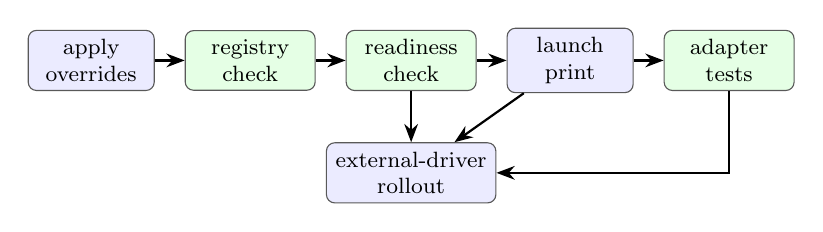
\begin{tikzpicture}[
  node distance=0.45cm and 0.38cm,
  auditstep/.style={rectangle,rounded corners=3pt,draw=black!65,fill=blue!8,
               minimum height=0.66cm,minimum width=1.6cm,font=\footnotesize,align=center},
  check/.style={rectangle,rounded corners=3pt,draw=black!65,fill=green!10,
               minimum height=0.66cm,minimum width=1.65cm,font=\footnotesize,align=center},
  arr/.style={-Stealth,thick}
]
  \node[auditstep] (overrides) {apply\\overrides};
  \node[check,right=of overrides] (registry) {registry\\check};
  \node[check,right=of registry] (ready) {readiness\\check};
  \node[auditstep,right=of ready] (print) {launch\\print};
  \node[check,right=of print] (tests) {adapter\\tests};

  \node[auditstep,below=0.65cm of ready] (rollout) {external-driver\\rollout};

  \draw[arr] (overrides) -- (registry);
  \draw[arr] (registry) -- (ready);
  \draw[arr] (ready) -- (print);
  \draw[arr] (print) -- (tests);
  \draw[arr] (ready) -- (rollout);
  \draw[arr] (print) -- (rollout);
  \draw[arr] (tests) |- (rollout);
\end{tikzpicture}
\caption{Audit path. Setup, readiness, command materialization, and tests isolate
integration failures before closed-loop rollouts.}
\label{fig:artifact_path}
\end{figure}

\section{Evaluation Protocol and Claim Boundary}

WOD2Sim should be evaluated as a closed-loop evaluation interface, not as a new driving
model. The minimal claim is execution validity: a WOD-style policy can be exposed as an
AlpaSim external driver, receive route and scene state through a stable contract, return
runtime trajectories, and produce auditable evidence. A stronger benchmark claim requires
executed scenes, baselines, and closed-loop failure analysis. Table~\ref{tab:eval_protocol}
summarizes the evaluation protocol supported by the artifact.

\begin{table}[t]
\centering
\small
\begin{tabular}{p{0.26\linewidth}p{0.33\linewidth}p{0.30\linewidth}}
\toprule
Category & Report & Purpose \\
\midrule
Baselines & open-loop WOD-style evaluation, replay or constant-velocity driver,
route-following driver, stock AlpaSim external-driver path, and WOD2Sim ablations without
route reconstruction or lifecycle hardening & show what closed-loop execution and the
adapter contract add beyond a simple API wrapper \\
Closed-loop metrics & collision rate, off-road rate, route progress, completion,
timeout rate, valid-frame ratio, sensor freshness, action latency, late-message rate, and
support-bundle validity & separate policy behavior from runtime and evidence failures \\
Scene coverage & straight, turn, lane-change, dense-traffic, occlusion, and route-merge
scenes across at least a small multi-scene set & support claims beyond a single recorded
scene \\
Failure taxonomy & route drift, stale observations, heading-error compounding, recovery
failure, lifecycle crashes, and audit invalidation & expose failures hidden by open-loop
log replay \\
\bottomrule
\end{tabular}
\caption{Evaluation protocol for claims built on WOD2Sim. The current release validates
the contract and records one closed-loop run; broader benchmark claims require larger
scene counts and baselines.}
\label{tab:eval_protocol}
\end{table}

The claim boundary is therefore precise: WOD2Sim bridges WOD-style policy
interfaces to AlpaSim closed-loop execution. It does not claim full Waymo scene
reconstruction, a new simulator, or a new autonomy model. That boundary is important
because a full Waymo-to-AlpaSim converter would need to reconstruct maps, actors, dynamic
agents, traffic lights, sensor setup, and dataset terms at a scope beyond this artifact.

\section{What Generalizes}

WOD2Sim is specific to this project, but the adapter pattern is not. The same
external-driver shape should transfer to other dataset-trained or benchmark-trained
trajectory policies that are not written as native AlpaSim drivers.

The reusable part is the boundary definition: preserve simulator route geometry at
prediction time; keep policy code independent of dataset protobufs and simulator message
internals; register policies through the existing \texttt{alpasim.models} mechanism;
separate base driver abstractions from optional heavyweight backends; handle late session
messages idempotently; and materialize launch state before rollout. Those choices let
very different policies share one closed-loop runtime. In this artifact, the reflex
policy, learned token policy, and direct actor planner all run through the same route
signal, resampling path, and launch system.

The result is therefore more than a WOD integration. It is a concrete reference for what
an AlpaSim external-driver adapter has to provide when the source policy was designed for
offline learning or log-based evaluation rather than for a persistent simulator service.

\section{Limitations}

WOD2Sim does not claim to reconstruct the full WOD world state inside AlpaSim. Its
primary claim is execution compatibility: making WOD-style and project policies run as
native AlpaSim drivers. Richer traffic reconstruction, broader WOD subset release,
dataset-terms packaging, and standard public baselines are natural next steps. The
current contract exposes the important systems boundary: route geometry, trajectory
timing, plugin loading, deployment, and simulator-driver interaction.

\section{Conclusion}

WOD2Sim extends AlpaSim's external-driver contract for WOD-style trajectory policies.
The extension preserves route geometry at prediction time, decouples external plugin
discovery from unselected built-in backends, treats late session messages idempotently,
and records launch state before rollout. Project policies then run as ordinary
\texttt{alpasim.models} plugins over a compact policy-facing signal. The result is a
closed-loop harness for minimal-shot, learned token, and actor-aware planning policies,
and a reference contract for building additional AlpaSim adapters.

\bibliography{paper}

\end{document}
